%%%%%%%%%%%%%%%%%%%%%%%%%%%%%%%%%%%%%%%%%%%%%%%%%%%%%%%%%%%
% --------------------------------------------------------
% Tau
% LaTeX Template
% Version 2.4.3 (01/09/2024)
%
% Author: 
% Guillermo Jimenez (memo.notess1@gmail.com)
% 
% License:
% Creative Commons CC BY 4.0
% --------------------------------------------------------
%%%%%%%%%%%%%%%%%%%%%%%%%%%%%%%%%%%%%%%%%%%%%%%%%%%%%%%%%%%

\documentclass[9pt,a4paper,twoside]{tau-class/tau}
\usepackage[english]{babel}
\usepackage{multirow}

%----------------------------------------------------------
% TITLE
%----------------------------------------------------------

\journalname{Aprenentatge Computacional}
%% TODO: Optional, you can set a fancier title if you like
\title{Titanic Survival Prediction using Classical and Machine Learning Models}

%----------------------------------------------------------
% AUTHORS, AFFILIATIONS AND PROFESSOR
%----------------------------------------------------------

%% TODO: Set your names here
\author[a,1]{Oriol Jiménez Asensi}
\author[b,2]{Fèlix Sáiz von Fraunberg}
\author[c,3]{Eduardo Pérez Motato}
\author[d,4]{Roger Guitart Casals}

%----------------------------------------------------------

\affil[a]{1641014}
\affil[b]{1620854}
\affil[c]{1709992}
\affil[d]{1711342}

%----------------------------------------------------------
% FOOTER INFORMATION
%----------------------------------------------------------

\institution{Universitat Autònoma de Barcelona}
\footinfo{Class Project}
\theday{October 27, 2025}
\leadauthor{Group 15} 		%% TODO: Set your group ID here
\course{Aprenentatge Computacional}

%----------------------------------------------------------
% ABSTRACT AND KEYWORDS
%----------------------------------------------------------

\begin{abstract}    
	%% TODO: Change this default abstract into something nice that describes your work.
	%% Keep it below 300 words.
In this project, we analyze the Titanic dataset to predict passenger survival using classical and machine learning models. After data cleaning and feature engineering, we evaluate Logistic Regression, SVM, and Random Forest classifiers through cross-validation. The Random Forest achieved the best accuracy (0.83), showing robust performance with balanced precision and recall.\end{abstract}

%----------------------------------------------------------

%% TODO: Set appropriate keywords for your report.
\keywords{a, b, c, d}

%----------------------------------------------------------

\begin{document}
	%% Do NOT change any of this. Line numbers should be kept.
    \maketitle 
    \thispagestyle{firststyle} \tauabstract 
    \tableofcontents
    \linenumbers 
    
%----------------------------------------------------------

\section{Exploratory data analysis}

    La base de dades consta de 12 columnes, incloent la variable target. Aquesta variable, anomenada Survived, és binària i conté 549 mostres falses i 342 mostres verdaderes, indicant que està relativament equilibrada.

    \begin{table}[H]
		\centering
		\caption{Tipus de les variables independents}
		\label{tab:tipus_variables}
		\begin{tabular}{cc}
			\toprule
			\textbf{Nom} & \textbf{Tipus}\\
			\midrule
			PassengerId & enter\\
            Pclass & categorica\\
            Name & cadena de caracters\\
            Sex & binaria\\
            Age & punt flotant\\
            SibSp & enter\\
            Parch & enter\\
            Fare & punt flotant\\
            Cabin & cadena de caracters\\
            Embarked & categorica\\ 
			\bottomrule
		\end{tabular}			
	\end{table}

Pel que fa als NaNs, la mostra d'entrenament presenta 177 valors nuls a la columna Age, 687 a la columna Cabin i 2 a la columna Embarked. 

Fent una matriu de correlació al quadrat de les variables numèriques observem que Survived està relacionada amb Pclass, Sex, Fare. Age està relacionada amb Pclass i Pclass està molt relacionada amb Flare.

\begin{figure}[H]
    \centering
    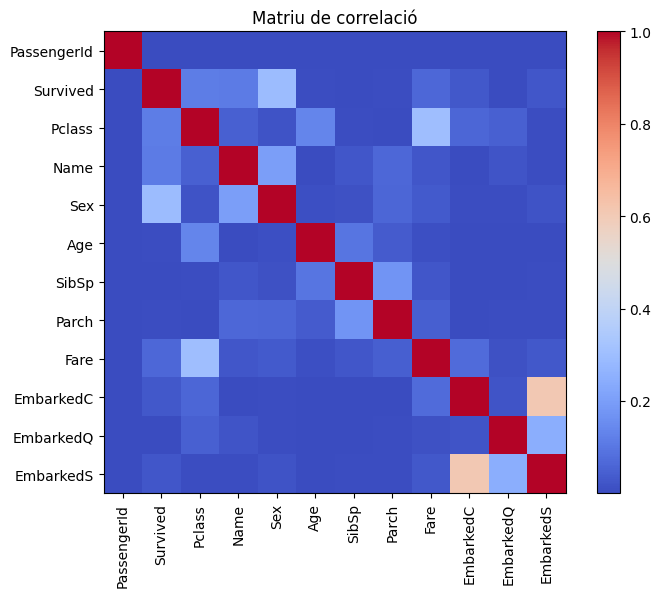
\includegraphics[width=0.4\textwidth]{correla.png}
    \caption{Matriu de correlació al quadrat de les variables numèriques}
    \label{fig:correlacio}
\end{figure}

Quant a les etiquetes de les variables categòriques (com amb la variable target), no sembla que les etiquetes estiguin prou poc representades per causar "problemes de categories rares".

\begin{table}[H]
		\centering
		\caption{Etiquetes d'Embarked}
		\label{tab:etiquetes_embarked}
		\begin{tabular}{cc}
			\toprule
			\textbf{Etiqueta} & \textbf{Nombre d'instàncies}\\
			\midrule
			S & 644\\
            C & 168\\
            Q & 77\\
            \bottomrule
		\end{tabular}			
	\end{table}

\begin{table}[H]
		\centering
		\caption{Etiquetes de Pclass}
		\label{tab:etiquetes_pclass}
		\begin{tabular}{cc}
			\toprule
			\textbf{Etiqueta} & \textbf{Nombre d'instàncies}\\
			\midrule
			1 & 216\\
            2 & 184\\
            3 & 491\\
            \bottomrule
		\end{tabular}			
	\end{table}
    
\section{Preprocessing}
    Les dades no estan normalitzades. Malgrat que les instàncies numèriques no semblen ser excessivament grans, considerem que normalitzar les dades sempre és una cosa positiva.
    En aquest cas, utilitzarem una estandarització Z. 
    PassengerId i Name semblen inútils a l'hora de realitzar la predicció. Malgrat això, sovint la longitud del nom és considerada una mostra de prestigi com es veu a l'aristocràcia, per això també hem decidit provar 
    d'afegir la mida del nom com a variable. Curiosament, a la matriu de correlació al quadrat es pot veure una correlació amb la variable target. 
    Per tractar les variables categoòriques, podem aprofitar la monotonietat de la variable Pclass per interpretar-ho com una variable numèrica i repartir Embarked en tres variables binàries. Aquestes evidentment apareixen correlacionades a la matriu de covariàncies. 
    En quant als Nans, els hem substituït per -1 a les variables numèriques (Age) i a Embarked simplement quedarà 0 en totes les categories.
    Considerem que no té sentit filtrar-los tenint en compte que al test set també n'hi ha i els necessitarem per fer la predicció.
    No hem realitzat pca perquè teniem molt poques variables i per tant era irrellevant.

\section{Metric Selection}
    Hem entrenat un model logístic a partir de les dades preprocessades i sense tocar hiper-paràmetres.
    Hem creat la matriu de confusió del model i hem provat l'accuracy, la f1\_score i l'average\_precission\_score.
    Despres hem realitzat la corba roc i la precission-recall curve. A partir d'aquí hem determinat que la variable target no està gaire descompensada, 
    utilitzarem l'accuracy\_score.

    \begin{figure}[H]
        \centering
        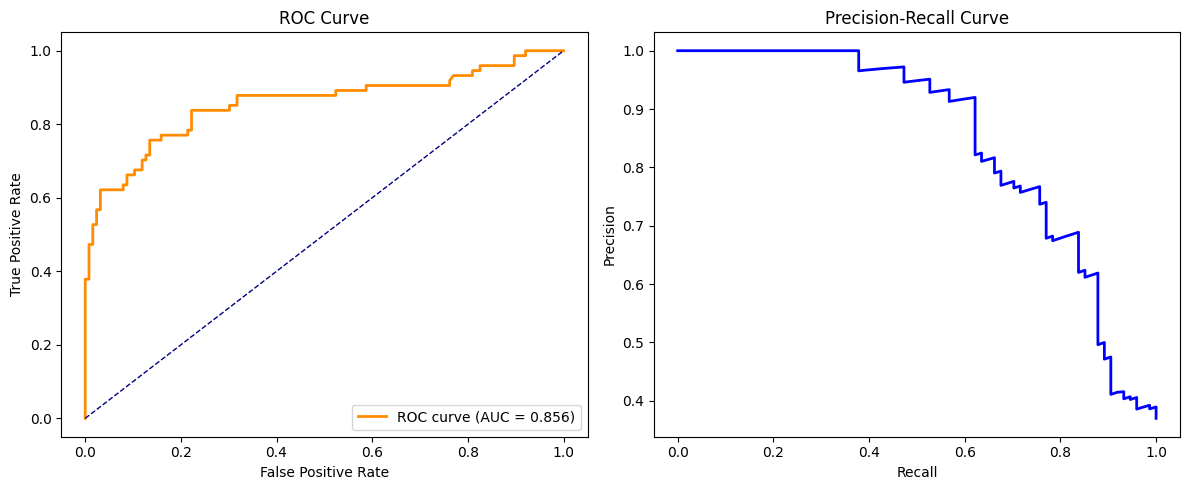
\includegraphics[width=0.4\textwidth]{grafic.png}
        \caption{Corba ROC i Precission-Recall Curve}
        \label{fig:grafic}
    \end{figure}
    \begin{table}[H]
        \centering
        \caption{Matriu de confusió (test)}
        \label{tab:confusion_matrix}
        \begin{tabular}{cc|cc}
            & & \multicolumn{2}{c}{\textbf{Prediccions}} \\
            & & \textbf{0} & \textbf{1} \\
            \cline{3-4}
            \multirow{2}{*}{\rotatebox[origin=c]{90}{\textbf{Reals}}} 
            & \textbf{0} & 105 & 21 \\
            & \textbf{1} & 17 & 57 \\
        \end{tabular}
    \end{table}

\section{Model Selection amb validació creuada}
    Hem entrenat els següents models per a triar quin encerta més, aquestes han estat SVM i LogisticRegrsion ja que són els que s'han fet a classe i com a 3r hem triat el RandomForests, ja que el coneixem de l'assignatura de OOP.
    Els accuracy scores dels models amb hyper-paràmetres per defecte són:
\begin{table}[H]
		\centering
		\caption{Accuracy scores dels models}
		\label{tab:accuracy_scores}
			\begin{tabular}{cc}
			\toprule
			\textbf{Model} & \textbf{Accuracity-score}\\
			\midrule
			SVM & 0.813722\\
            RandomForest & 0.804733\\
            LogisticRegrsion & 0.775551\\
            \bottomrule
		\end{tabular}			
	\end{table}
    Malgrat que el temps d'entrenament per aquesta base de dades és negligible, si l'escalèssim el que donaria millors resultats seria el logistic (0.011358s) seguit de el SVM(0.093215s) i RF (0.588249s).
    En quant a la cerca d'hiperparàmetres ens hem plantejat utilitzar grid search (GridSearchCV) però era molt costós i ens preocupava que, degut la petita mida de la mostra, es produís overfiting implícit. Per tant hem acabat utilitzant random search (RandomizedSearchCV) amb 45 iteracions per model.
    El que ha donat millors resultats pels models ha sigut:
\begin{table}[H]
    \centering
    \caption{Resultats de la cerca d'hiperparàmetres dels models}
    \label{tab:hiperparametres}
    \begin{tabular}{lcc}
        \toprule
        \textbf{Model} & \textbf{Accuracy mitjà} & \textbf{Temps (s)} \\
        \midrule
        RandomForest & 0.829364 & 9.052283 \\
        SVM & 0.821543 & 2.532295 \\
        LogisticRegression & 0.785619 & 1.517158 \\
        \bottomrule
    \end{tabular}
\end{table}

\noindent\footnotesize\textit{Millors hiperparàmetres utilitzats:}
\begin{itemize}
    \item \textbf{RandomForest}: \texttt{\{'n\_estimators': 100, 'min\_samples\_split': 5, ...\}}
    \item \textbf{SVM}: \texttt{\{'kernel': 'rbf', 'gamma': 0.1, 'C': 1.6681005...\}}
    \item \textbf{LogisticRegression}: \texttt{\{'solver': 'liblinear', 'penalty': 'l1', 'C': ...\}}
\end{itemize}
\section{Anàlisi Final}
La mètrica principal (Accuracy = 0.89) mostra un bon rendiment global. En un context pràctic, el model podria servir per assignar una probabilitat de supervivència i prioritzar recursos o suports segons risc. També podria usar-se com a eina d’anàlisi per entendre quines variables influeixen més en la supervivència.

Es podria millorar per exemple, extreure el títol del nom o crear la mida de la família, imputacions més precises dels valors nuls i ajust d'hiperparàmetres amb més iteracions.

\section{Acknowledgements}

Tau \LaTeX template built by Guillermo Jimenez.

%----------------------------------------------------------

\addcontentsline{toc}{section}{References}
\printbibliography

%----------------------------------------------------------

\end{document}